\section{Nebulas Rank}
\label{sec:rank}

\subsection{Nebulas Rank Overview} \label{subsec:value}
Currently the Blockchain technology and community have grown into a large scale ecosystem. However, people's perception of Blockchain world is still relatively flat; there is no reasonable way to evaluate the entity, such as user's address, on the blockchain yet. Therefore, we try to come up with a universal value measurement. By mining activities occurs on chain, the value of every entity (address) is able to be quantified as \textbf{Nebulas Rank}. \textbf{Nebulas Rank} is aimed at two goals:
\begin{itemize}
	\item As a native value measurement, \textbf{Nebulas Rank} could become core algorithms for many fundamental scenarios, such as consensus (see \refsec{}), DIP (see \refsec{}) and Blockchain search engine (see \refsec{}), etc.
	\item \textbf{Nebulas Rank} could inspire various value measurements, as well as deeper insights into the blockchain ecosystem.
\end{itemize}
Based on the goals above, we define the value measurement of \textbf{Nebulas Rank} to be three-fold:
\begin{itemize}
	\item Liquidity, the frequency and scale of transactions, is the first dimension that \textbf{Nebulas Rank} considers. Essentially, by means of capital liquidity, financial activity can promote efficient configuration of social resources and promote economy development. Blockchain established a value network. Thus more transactions and larger transaction scale produce better liquidity, and better liquidity further increases more transactions and larger transaction scale, forming a complete mechanism of positive feedback.
	\item Propagation, the scope and depth of liquidity, is the second dimension that \textbf{Nebulas Rank} considers. In social network, the propagation property, i.e. speed, scope and depth of information propagation, is key measurement indicating network quality and users growth. We see same pattern in the Blockchain world. Better propagation means wider and deeper assets liquidity, which improves the quality of assets in the Blockchain world, and increases the scale of assets.
	\item Interoperability is the third dimension that \textbf{Nebulas Rank} considers. During the early stage of Internet, there were just simple websites and isolated information. Nowadays, all kinds of Internet platforms begin to interact with each other and the small information islands begin to disappear. This tendency could be understood as a process of recognizing information from higher dimensional perspective. We believe that Blockchain world also follows the same roadmap, whose development will be faster. There will be more information of users' assets, smart contract and DApp. And also, there will be more frequent interactions among them. Thus better interoperability will become more important.
\end{itemize}

We choose transaction records on chain as source data for \textbf{Nebulas Rank}. Because comparing with real world, the "trajectory" in Blockchain world is more clear and trustworthy: the transaction data on chain loyally records every transferring among addresses and invoking of "smart contracts". But it is not trivial to design rank algorithm for Blockchain transaction data, since comparing with real world, the transactions in Blockchain world are naturally anonymous and bears larger data scale. So we depict three properties for \textbf{Nebulas Rank}:
\begin{itemize}
	\item Truthful. An entity must pay reasonable effort to improve its rank, which assures that the algorithm can identify trusted valuable users. On one hand, in scenarios like consensus and DIP, truthful ranking encourages users to contribute truthfully in order to realize positive feedback. On the other hand, truthful result provides meaningful hierarchy representation of all users, which will be more helpful for decision makers;
	\item Computable. As a fundamental field, \textbf{Nebulas Rank} of every user should be accessible instantly and thus requires low computational complexity;  
	\item Reproducible. Due to consensus and DIP, the running result of \textbf{Nebulas Rank} algorithm needs to be identical by any client.
\end{itemize}

Next we design basic framework of \textbf{Nebulas Rank}. First, transaction records are represented in the form of graph. By the definition of transaction graph (entity graph), every node is mapped to one entity, and each edge represents the transferring between two entities\cite{Tschorsch2015}. Transaction graph embeds the fact that money transferring among users leads to assets flowing, which helps to represent the concepts of liquidity and propagation defined before. Meanwhile, the form of graph is convenient to formulate the interoperability among contracts. With the derived transaction graph, we rank nodes by their network centrality. In the scenario of \textbf{Nebulas Rank}, LeaderRank\cite{Chen2013}\cite{Li2014} is a more reasonable measurement and outperforms PageRank and NEM\cite{nem}.。

\subsection{Transaction Graph} \label{subsec:txg}
This subsection introduces how to derive transaction graph from transaction history.

First, we take effective transferring among  individual addresses during the past $T$ (generally $T$ is the number of blocks in a month) blocks, denoted by $T_{xs}$:
\begin{align}
T_{xs} = \{(s,t,\tau, a)| \tau = \#CurrentBlock-T \dots \#CurrentBlock \land a > 0 \}
\end{align}
, where $s$, $t$ and $a$ are source address, target address and transfer amount.

Then based on $T_{xs}$, a directed weighted simple graph is constructed, denoted as $G=(V, E, W)$, where node set, edge set and edge weights are denoted by $V$, $E$ and $W$ respectively. Additionally, let $N = |V|$,$M = |E|$. For simplicity, every node is represented by an integer between $1$ and $N$.

Every node represents an individual account's address, and each edge represents the intensity between two addresses. Edges are directed and are assigned with weight $w_e$ aggregating top $K$ amounts of all related transactions:
\begin{align}\label{formula:edgeweight}
w_e = \sum_{i=1}^K a_i, s.t. a_i \in \{a|(s,t,\tau,a) \in T_{xs} \} \land a_1 \geq a_2 \dots
\end{align}

\begin{figure}[h]
\centering
	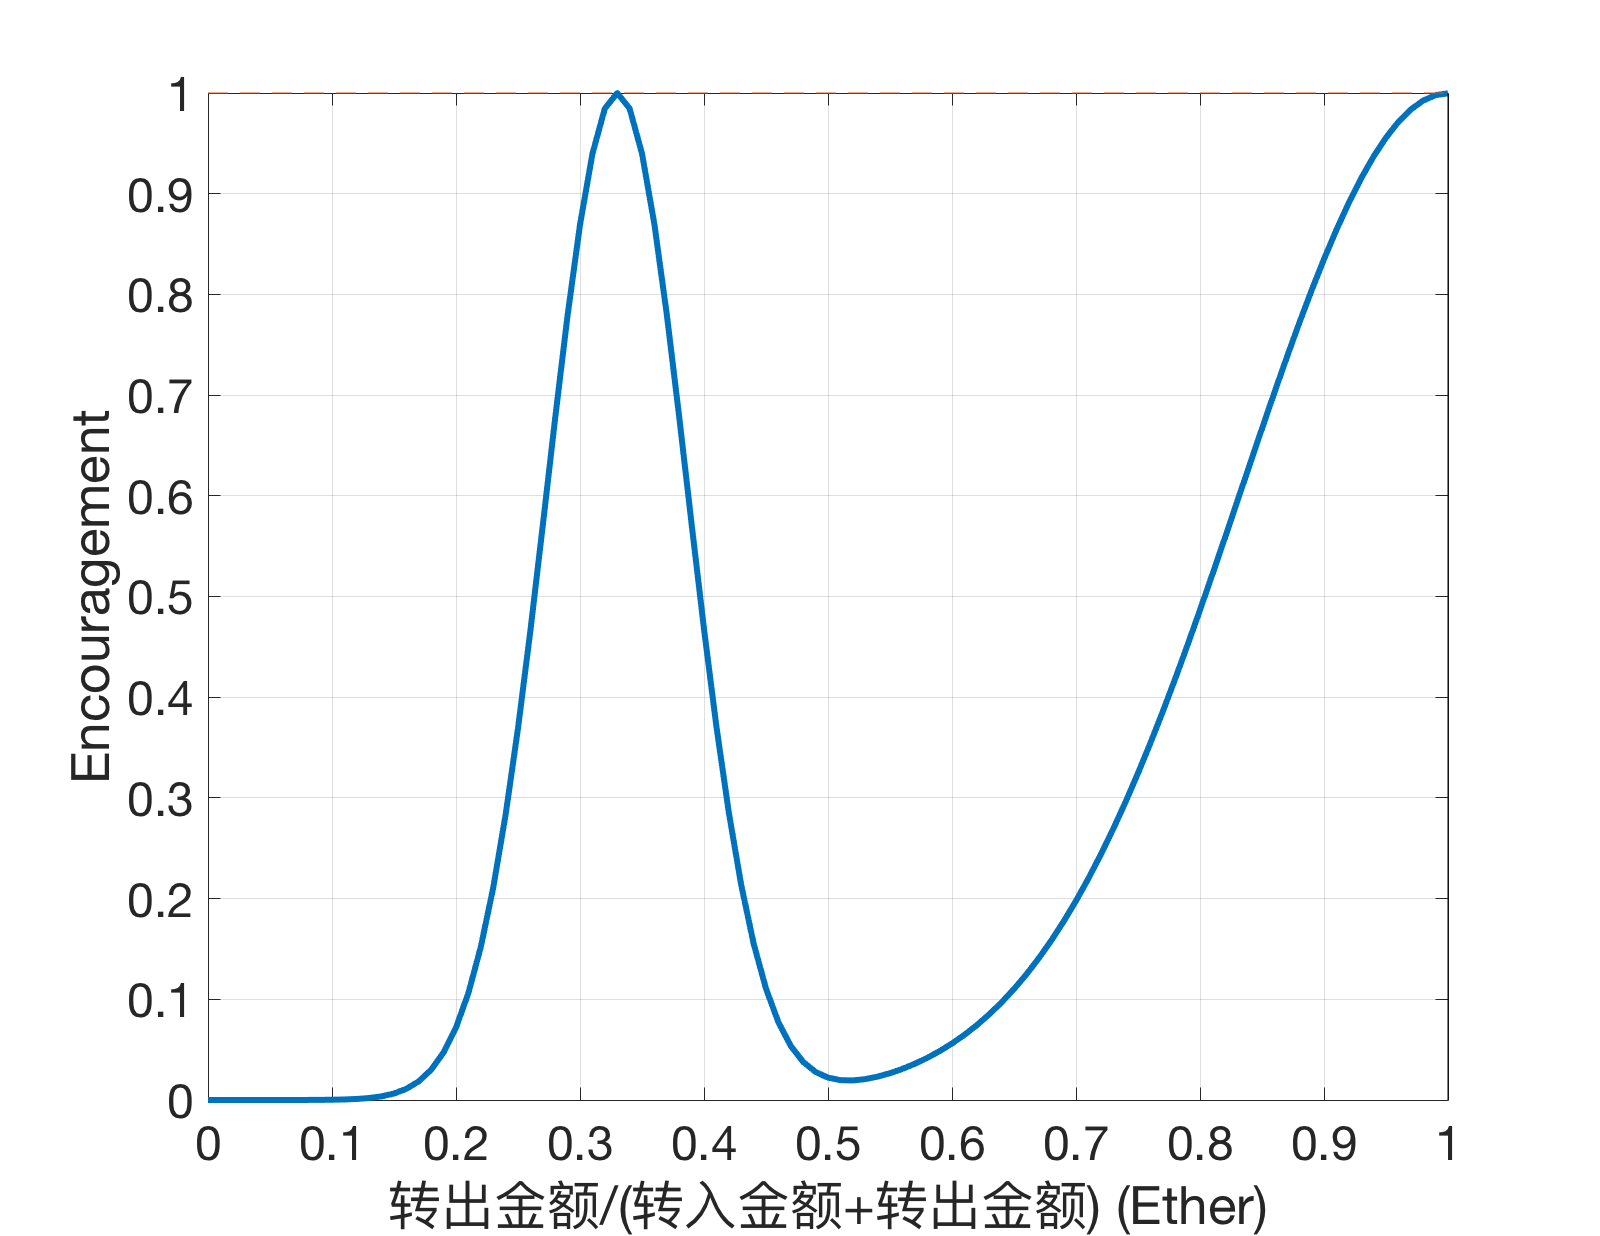
\includegraphics[width=0.55\textwidth]{figs/encouragement.png}
	\caption{Encouragement Function}\label{fig:encouragement}
\end{figure}

Then for each node, according to its in-transfers and out-transfers during the past $T$ blocks, we compute its "coinage", denoted by $C_v$; also, based on an "encouragement function" shown in \reffig{fig:encouragement}, we compute its encouraged value, denoted by $E_v$.\footnote{Encouragement function can be represented as a linear combination of two normal distributions, which outputs peak value when the money transferred out is zero or of some ratio of the amount transferred in.} And then the edges' weight is reduced by their target node's $C_v$ and $E_v$.

Finally, we take the largest weakly connected component of the whole graph, only remaining nodes belonging to this component.

The graph derivation described above contributes to the "truthful" property defined at \refsec{subsec:value}, the evidence of which is shown in \refsec{subsec:robust}.

We collect data on Ethereum Main Net Blockchain. It starts at \#3629091(roughly on May 1st, 2017) and ends at\#3800775(roughly on May 31st, 2017), containing $171,684$ transactions in total. Let $T=171,684$, $K=2$, we construct the transaction graph according to the method introduced by this subsection, and its visualization is shown as \reffig{fig:wgc}. Some nodes are labeled by tags in Etherscan\cite{etherscan}, and all nodes are resized by their degree. It could be observed that some famous exchanges usually interacts with more accounts than others. Besides, the identities of some addresses who contributes a lot transactions still remains unknown. 

\begin{figure}[h]
	\centering
	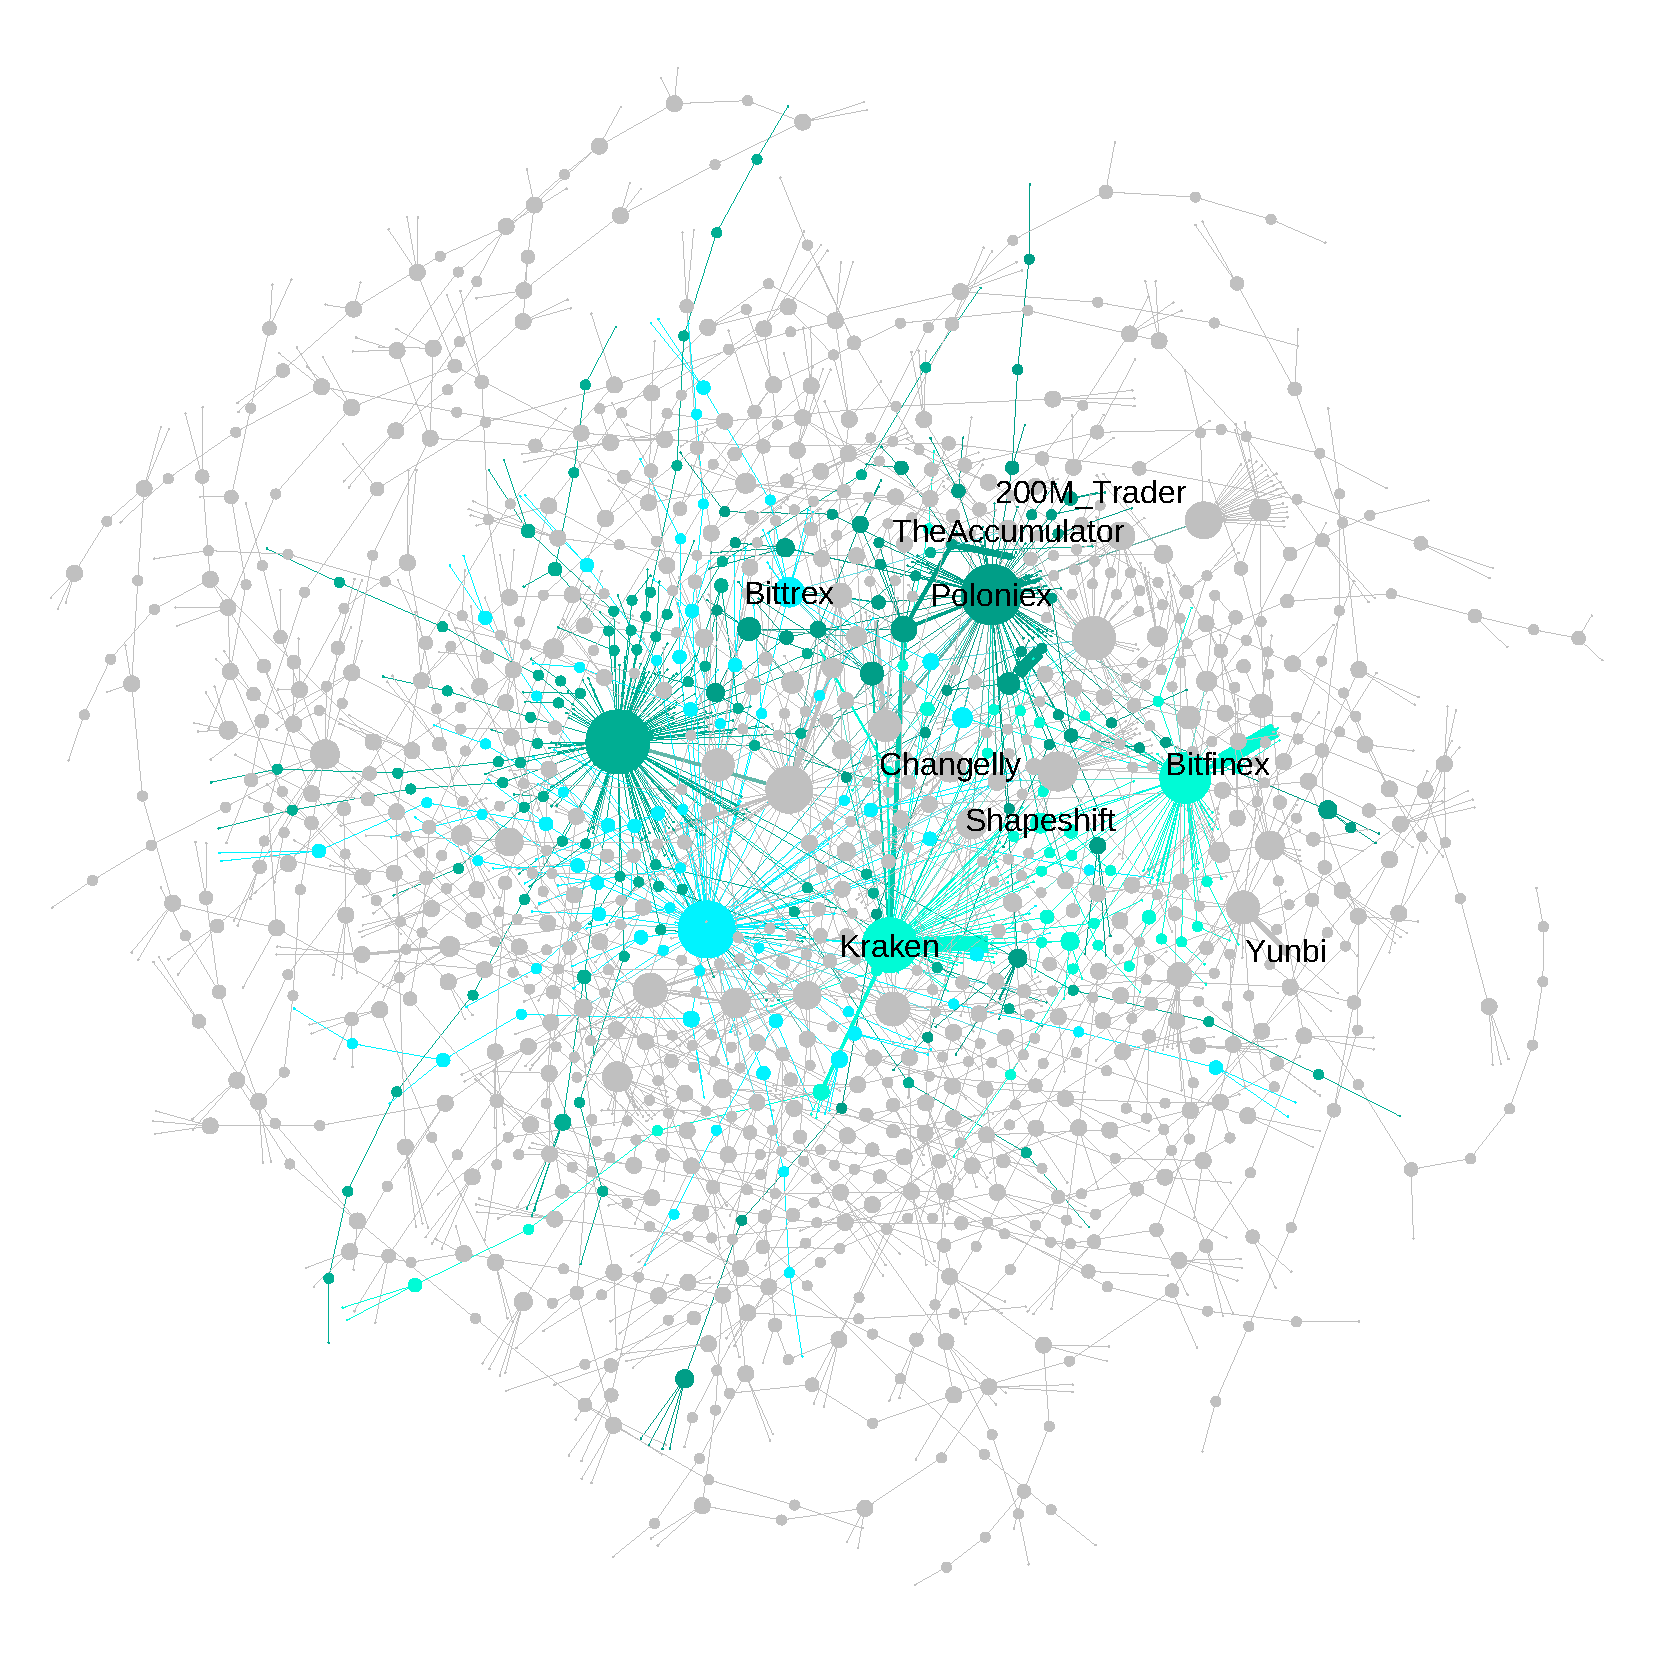
\includegraphics[width=0.85\textwidth]{figs/wgc1.png}
	\caption{Transaction Graph (Partly) Visulazation }\label{fig:wgc}
\end{figure}

\subsection{Ranking Algorithm} \label{subsec:leaderrank}
This subsection introduces how to rank nodes by their importance in the derived transaction graph.

We adopt LeaderRank\cite{Chen2013}\cite{Li2014} as the main method. First, a ground node is added into the transaction graph, denoted by $\mathcal{G}$ and numbered as $N+1$. Then we establish double link between the ground node and every other node, weighting by the following formula:
\begin{align}\label{formula:weight1}
	\forall v \in V, w_{(v, \mathcal{G})} = \alpha A_v
\end{align}
\begin{align}\label{formula:weight2}
\forall v \in V,  w_{(\mathcal{G}, v)} = \beta B_v
\end{align}
, where 
\begin{align}
	\forall v \in V, A_v = \{ \sum_{(u,v)\in E} w_{(u,v)} - \sum_{(v,u) \in E} w_{(v, u)}, 0 \} + \lambda C
\end{align}
\begin{align} \label{formula:b}
\forall v \in V,  B_v =  \sum_{(u,v) \in E} w_{(u,v)} + \mu C
\end{align}
\begin{align}
	C = median\{w_e| e \in E\}
\end{align}

$\alpha, \beta, \mu, \lambda$ are parameters. The weighting scheme can be understood as that, nodes with more in-degree receive more in-link from the ground node; nodes with more absolute income, i.e. in-degree minus out-degree, outputs stronger link into the ground node. 

The running process of LeaderRank is similar with PageRank, which could be understood as computing the convergence state of a Markov process. What is different is that, after adding the ground node, it does not need to consider the damping factor of PageRank\cite{Brin2010}\cite{page1999pagerank} anymore. That is, after constructing matrix $H$ according to formula (\ref{formula:matrix}), the computing process is iterated until convergence, as formula (\ref{formula:iteration}) shows, with initial settings defined by formula (\ref{formula:init}). Finally the rank score of ground node is distributed evenly to every other node, which yields the final score for every node.
\begin{align} \label{formula:iteration}
	P^{t+1} = H \times R^{t}; P^1=[\frac{1}{N}, \frac{1}{N}, \dots, \frac{1}{N}, 0]^T
\end{align}
\begin{align} \label{formula:matrix}
	h_{ij} = \frac{w_{(j,i)}}{\sum_k w_{(j,k)}}
\end{align}
\begin{align} \label{formula:init}
\forall v \in V, P^*_v \leftarrow P^*_v + \frac{P^*_{\mathcal{G}}}{N}
\end{align}

We suppose that LeaderRank can satisfy the value measurements and algorithm property defined in \refsec{subsec:value}.
\begin{itemize}
	\item The result of LeaderRank can be understood as the flux on each node in the dynamic equilibrium of money exchange network, which matches \textbf{Nebulas Rank}'s value measurement of "liquidity", "propagation" and "interoperability";
	\item The weighing scheme defined by formula (\ref{formula:weight2}) and (\ref{formula:b}) makes it more difficult to attack (see discussion in \refsec{subsec:robust}), which satisfies "truthful" property;
	\item LeaderRank can be computed by power iteration. Since the network is very sparse, the complexity of matrix computation should not be high, which satisfies the properties of "computable" and "reproducible".
\end{itemize}


\subsection{Manipulation Resistance}\label{subsec:robust}
Truthfulness, i.e. the ability of resisting manipulation, is the most and challenging goal of \textbf{Nebulas Rank}. Some manipulation methods are as follows:
\begin{enumerate}
	\item Loop transfer. The attacker attacker transfers along a loop topology, which allows the same money flow over same edges repeatedly. By this mean, the attacker hopes to raise the weight of related edges;
	\item Transfer to random addresses, so that the out-degree of sybil node increases;
	\item Form an independent network component with addresses controlled by the attacker. So the attacker can pretend to be a central node;
	\item Interact with authoritative Exchange service addresses frequently, i.e. transfer the same money in and out an authoritative Exchange service address repeatedly, so that the attacker can acquire better structural position in the network.
\end{enumerate}

\textbf{Nebulas Rank} mitigates manipulation through the following mechanism:
\begin{itemize}
	\item Due to sliding windows of $T$ blocks, the attacker cannot increase its rank in short term;
	\item Since the edge weight is decided by the highest amount of related transactions, transferring along a loop topology cannot increase the edge weight unlimitedly. Meanwhile, from the sampled data described in \refsec{subsec:txg}, $91\%$ of edges corresponds with less than 2 transactions respectively. Thus $K=2$ is a reasonable choice to remain the intensity information on edges while being resistance to loop transfer;
	\item In order to have higher "coinage", the users needs to let money stay in their address for a while, which slows down the attacking speed;
	\item In order to get the maximum "encouragement value", as is shown in \reffig{fig:encouragement}, the account need to keep all income or transfer out only a small ratio of it. So when forging money flow, the attackers' deposit should decrease rapidly;
	\item Because only the giant component is selected, other independent components including the forged one will be filtered out as noise. From the sampled data described in \refsec{subsec:txg}, there are $453,285$ nodes and $970,577$ edges, with $1,169$ components. In the biggest component, there are $449,746$ nodes, about $99.2\%$ of all. In the second biggest component, there are just $133$ nodes, about $0.03\%$ of all. Thus taking the giant component can remain normal part of network as much as possible while filtering noise part out;
	\item Comparing with webpage ranking algorithm such as PageRank and NCDawareRank\cite{Nikolakopoulos2013}, the mechanism defined by formula (\ref{formula:weight2}) and (\ref{formula:b}) is more "conservative" to nodes with low income. That is, nodes with low in-degree gets weaker links from the ground node. In the blockchain transaction graph, nodes with low income are more likely to be created, and transferring to other random nodes cannot raise in-degree, either. So \textbf{Nebulas Rank} can increase the difficulty of manipulation.
\end{itemize}

接下来,基于2017年5月份Ethereum的交易图(见\refsec{subsec:txg}),我们展示一系列结论。

首先,我们列出\textbf{Nebulas Rank}排名部分地址,如表\ref{table:nr}所示\footnote{备注来源: Etherscan\cite{etherscan}},可以看出,交易所账户以及部分交易吞吐量较大地址的排名较为靠前。

\newpage

\begin{table}[!htbp]
\centering
\caption{\textbf{Nebulas Rank}排名前$10$名及部分其他地址}
\label{table:nr}
\begin{tabular}{llllll}\toprule
排名 & 地址                                                                                    & Nebulas Rank & 备注          & 转出金额(Ether) & 转入金额(Ether) \\
1  & \begin{tabular}[c]{@{}l@{}}0x267be1c1d684f78cb4f\\ 6a176c4911b741e4ffdc0\end{tabular} & 0.449275     & Kraken\_4   & 3214232.06  & 350008.00   \\
2  & \begin{tabular}[c]{@{}l@{}}0xd4c5867cec094721aab\\ c3c4d0fd2f2ac7878c79a\end{tabular} & 0.093798     &             & 58000.00    & 100947.00   \\
3  & \begin{tabular}[c]{@{}l@{}}0x027beefcbad782faf69f\\ ad12dee97ed894c68549\end{tabular} & 0.049277     & QuadrigaCX  & 207440.11   & 65606.40    \\
4  & \begin{tabular}[c]{@{}l@{}}0x0ee4e2d09aec35bdf08\\ 083b649033ac0a41aa75e\end{tabular} & 0.046831     &             & 56465.00    & 60087.96    \\
5  & \begin{tabular}[c]{@{}l@{}}0xc257274276a4e539741\\ ca11b590b9447b26a8051\end{tabular} & 0.037628     &             & 1071105.93  & 1434106.72  \\
6  & \begin{tabular}[c]{@{}l@{}}0xa53e0ca7d246a764993\\ f010d1fde4ad01189f4e6\end{tabular} & 0.033488     &             & 7764.68     & 3201.00     \\
7  & \begin{tabular}[c]{@{}l@{}}0xf259e51f791e9ed26e8\\ 9b6cae4a7c6296bfbd0b8\end{tabular} & 0.033481     &             & 3307.00     & 7731.30     \\
8  & \begin{tabular}[c]{@{}l@{}}0xf195cac8452bcbc836a\\ 4d32cfb22235af4ac1e9c\end{tabular} & 0.026343     &             & 10863.87    & 2315.69     \\
9  & \begin{tabular}[c]{@{}l@{}}0x94435d12c51e19d5b5c\\ 8656763f9069d37791a1a\end{tabular} & 0.024970     &             & 12938.58    & 15858.90    \\
10 & \begin{tabular}[c]{@{}l@{}}0x7580ba923c01783115d\\ 79975d6a41b3d38eff8d5\end{tabular} & 0.021670     &             & 263000.00   & 364793.49   \\
16 & \begin{tabular}[c]{@{}l@{}}0xcafb10ee663f465f9d10\\ 588ac44ed20ed608c11e\end{tabular} & 0.004995     & Bitfinex\_1 & 360000.00   & 1435858.40  \\
51 & \begin{tabular}[c]{@{}l@{}}0xd94c9ff168dc6aebf9b\\ 6cc86deff54f3fb0afc33\end{tabular} & 0.000868     & yunbi\_1    & 1179224.74  & 1202539.53  \\
64 & \begin{tabular}[c]{@{}l@{}}0x70faa28a6b8d6829a4b\\ 1e649d26ec9a2a39ba413\end{tabular} & 0.000590     & Shapeshift  & 52501.81    & 651933.49   \\
\bottomrule
\end{tabular}
\end{table}
\newpage

接着,对比交易金额和\textbf{Nebulas Rank}的关系。由于区块链交易可以理解为“资金交换”类型的网络流,根据\textcite{Borgatti2005}的研究工作,节点的度,即邻接边权值之和,是适用于此类网络的一个合适的中心性测度。以每个节点为中心思考,度,即交易吞吐金额(转入转出金额的和),是节点一跳局部信息的体现,直接反映了对应地址的历史资金流量,因此应该作为衡量排名算法的基准。交易金额与\textbf{Nebulas Rank}的关系如\reffig{fig:nrio}所示:没有节点能够以较低的交易金额获取靠前排名,而交易金额较大的节点也要满足一定条件才能取得高的排名,这可以大致印证\textbf{Nebulas Rank}的可信性。

\begin{figure}[!htbp]
	\centering
	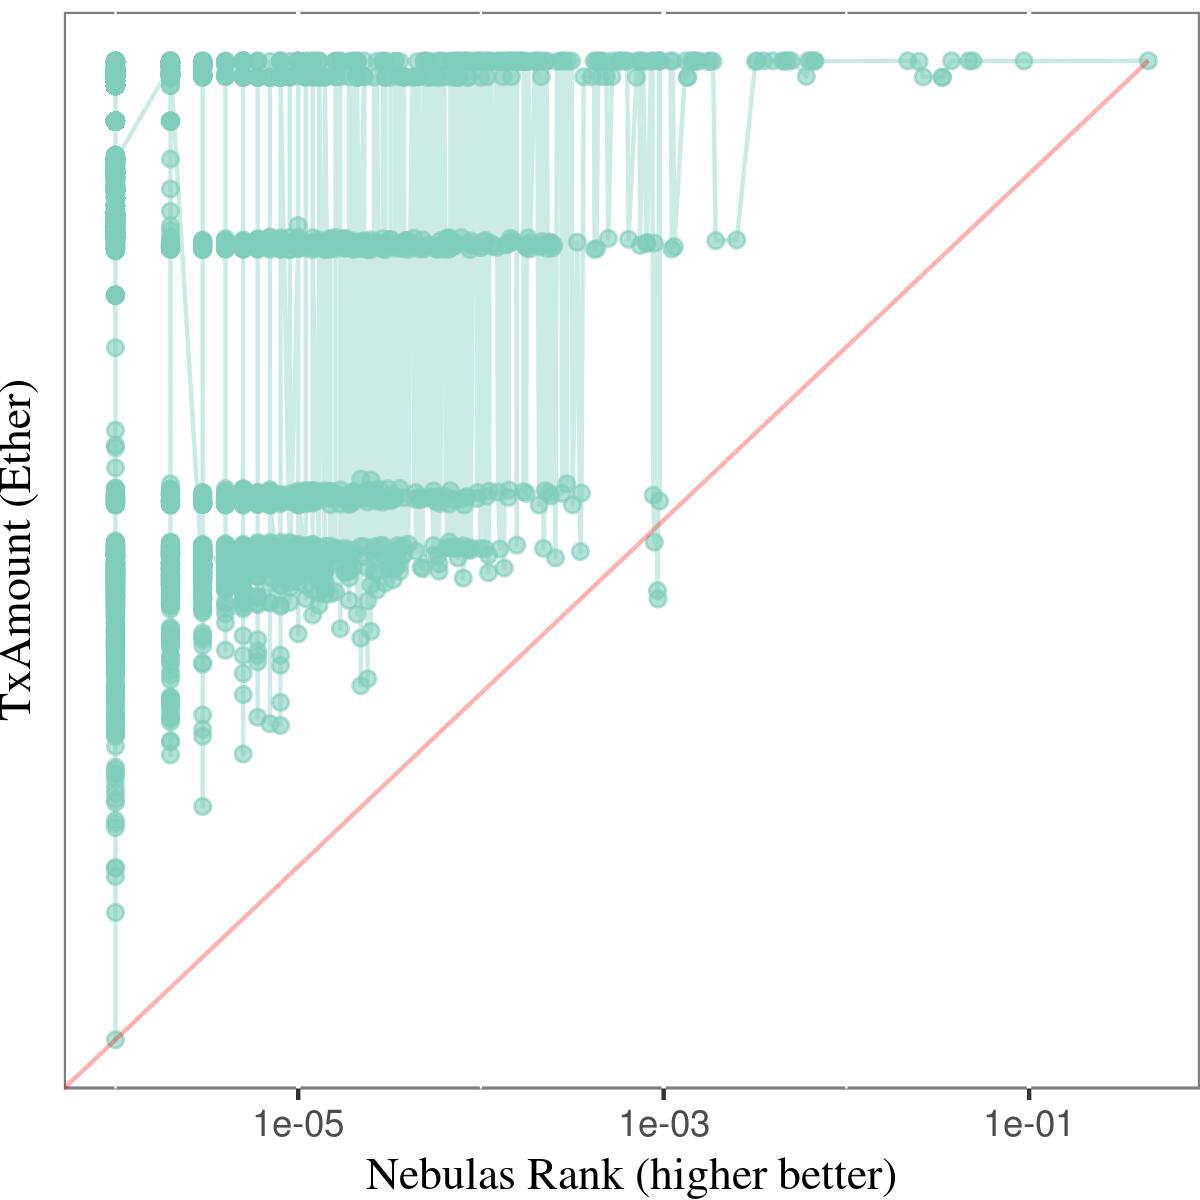
\includegraphics[width=0.40\textwidth]{figs/MAY_lr.png}
	\caption{Nebulas Rank v.s. 交易金额}\label{fig:nrio}
	\caption*{\footnotesize{横坐标为Rank值,纵坐标为交易金额,均为对数形式 \\ 图中斜线代表交易金额和rank值成正比例的情况 \\ 好的算法应该使得数据点尽可能少地落在斜线的右下方,以免低交易吞吐金额的节点取得好的重要性排名。}}
\end{figure}


在之前的部分,通过简单的分析可以推断,本小节开始所述的前三种攻击方式各自都可以被特定的处理手段有效过滤掉。因此最后,我们只需仿真最后一类攻击,攻击者选定某权威交易所节点,在排名计算周期内创造$X$次环形交易,每次交易时,攻击者先经由某新建地址向交易所节点转入$Y$Ether,之后经另一新建节点从交易所节点取出$Y$Ether,攻击方式示意图如\reffig{fig:loop}所示。此类攻击利用了某些交易所可以低成本建立转账链接的性质,虽然合法地址也可能和交易所频繁交易,但此类攻击的行为并未促进资产的有效流动,因此应该与合法行为在一定程度上区分开。

\begin{figure}[!ht]
	\centering
	%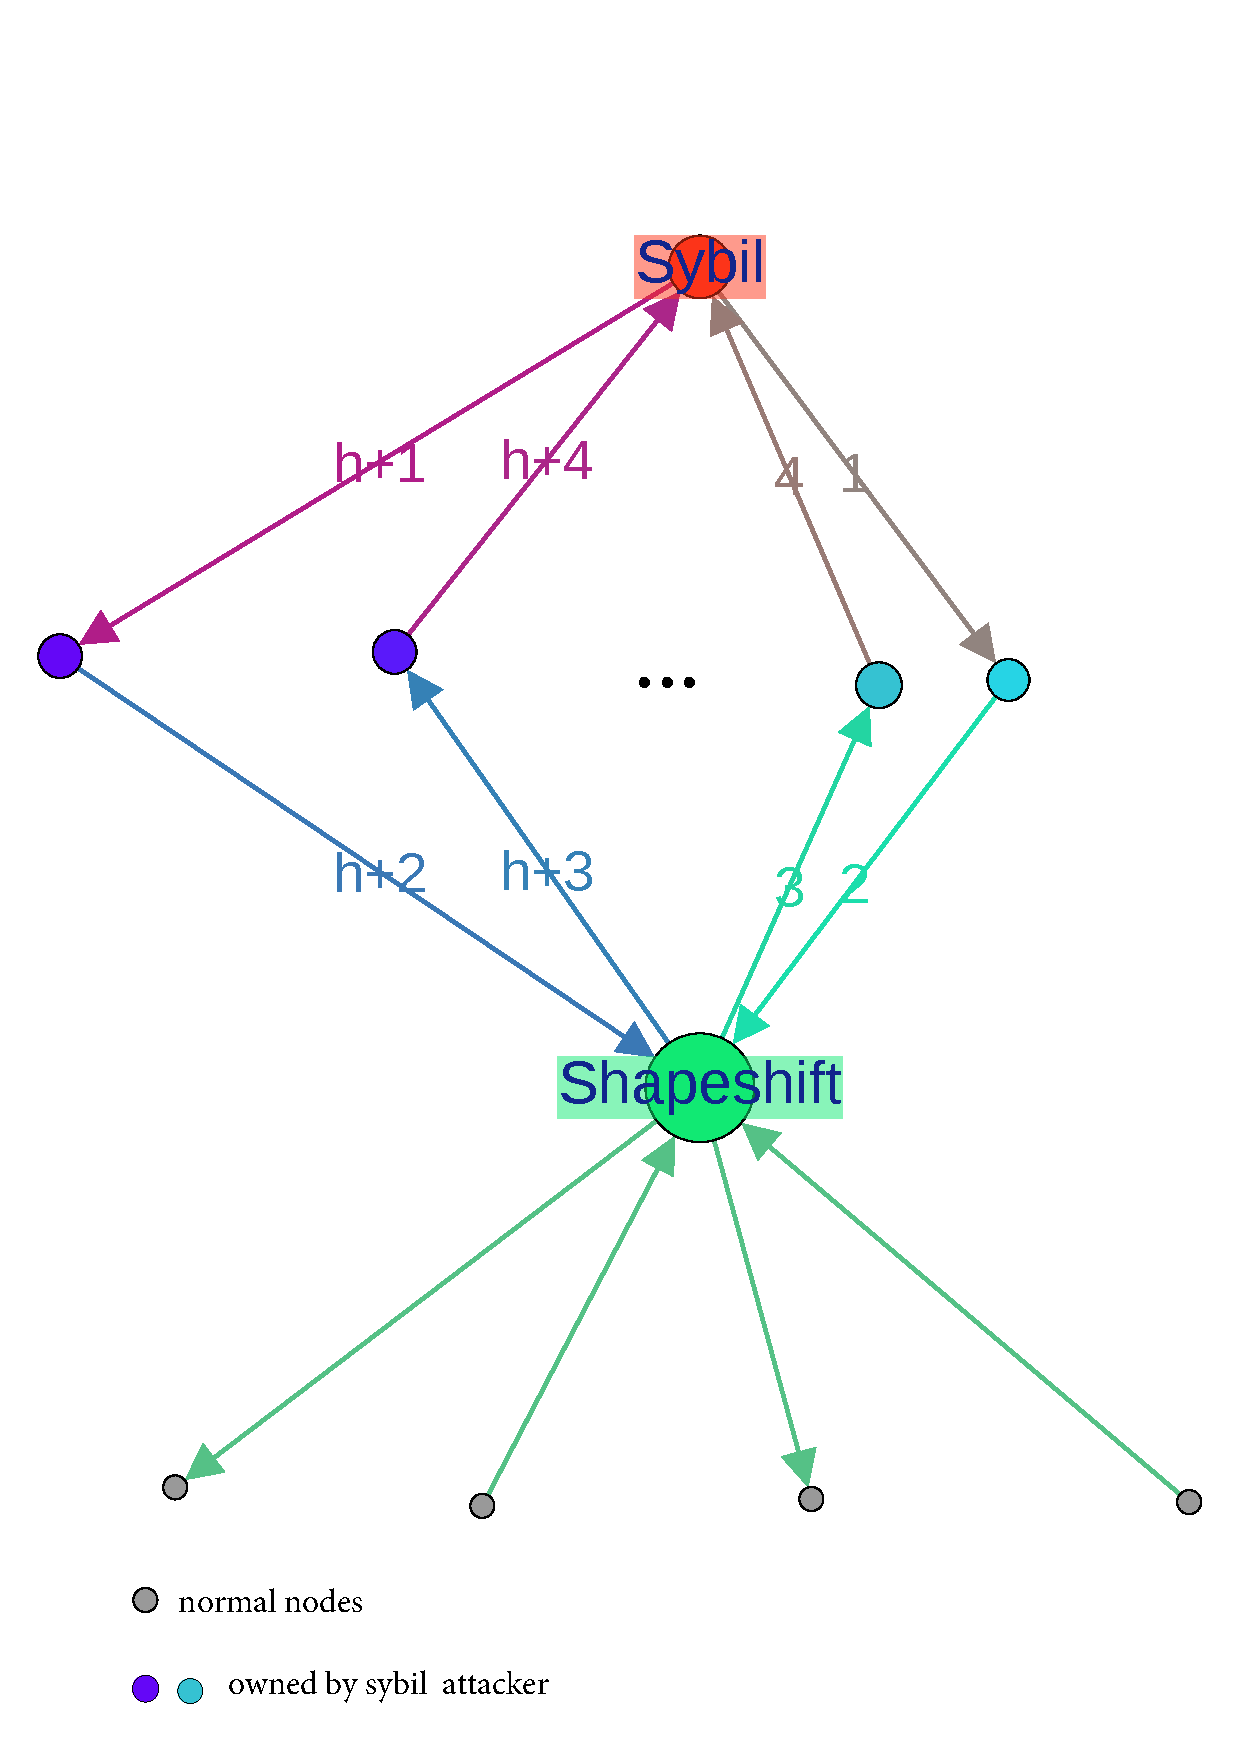
\includegraphics[width=0.35\textwidth]{figs/attack.pdf}
  \begin{tikzpicture}
  \pgfmathsetmacro{\YMD}{2}
  \pgfmathsetmacro{\XMD}{1.5}
\tikzset{
  hnode/.style={draw, circle, on grid, align=center, minimum height=2ex},
  base/.style={draw, circle, on grid, align=center, minimum height=4ex},
  sybil/.style={draw, circle, on grid, align=center, minimum height=4ex, fill=blue!20},
  normal/.style={draw, circle, on grid, align=center, minimum height=1ex, fill=gray!20},
  coord/.style={coordinate, on grid, node distance=6mm and 25mm},
}
%
\tikzset{>=stealth',
  every join/.style={->}, very thick}

       \node [base, fill=green!=20] (ss) at (0, 0) {} node[right
       = 1ex of ss] {Shapeshfit};

       \node (dot) at ($(ss.north) + (0, \YMD)$) {...};

       \node [sybil] (sy) at ($(dot.north) + (0, \YMD)$) {} node[right=1ex of
       sy]{Sybil};

       \node [hnode, fill=brown!50] (hh4) at($(dot.west) + (-\XMD, 0)$){};
       \node [hnode, fill=brown!50] (hh1) at ($(hh4.west) + (-\XMD, 0)$){};

       \node [hnode, fill=cyan!20] (h4) at ($(dot.east) + (\XMD, 0)$){};
       \node [hnode, fill=cyan!20] (h1) at ($(h4.east) + (\XMD, 0)$){} node
       [right = 1ex of h1]{owned by sybil attacker};

       \node [coord] (c) at($(ss.south) + (0, -\YMD)$) {};

       \node [normal] (n2) at ($(c.west) + (-\XMD, 0)$){};
       \node [normal] (n1) at ($(n2.west) + (-\XMD, 0)$){};
       \node [normal] (n3) at ($(c.east) + (\XMD, 0)$){};
       \node [normal] (n4) at ($(n3.east) + (\XMD, 0)$){} node [right=1ex of
       n4] {normal nodes};

       \draw[->, color=red] (sy) -- (hh1) node [midway, left]{h+1};
       \draw[->, color=red] (hh4) -- (sy) node [midway, right]{h+4};
       \draw[->, color=olive] (h4) -- (sy) node [midway, left]{4};
       \draw[->, color=olive] (sy) -- (h1) node [midway, right]{1};

       \draw[->, color=red] (hh1) -- (ss) node [midway, left]{h+2};
       \draw[->, color=red] (ss) -- (hh4) node [midway, right]{h+3};
       \draw[->, color=olive] (ss) -- (h4) node [midway, left] {3};
       \draw[->, color=olive] (h1) -- (ss) node [midway, right]{2};

       \draw[->] (ss) -- (n1);
       \draw[->] (n2) -- (ss);
       \draw[->] (ss) -- (n3);
       \draw[->] (n4) -- (ss);

\end{tikzpicture}

	\caption{将交易所纳入环形交易的攻击示意图}\label{fig:loop}
	\caption*{\footnotesize{图中给出了第1次和第h次环形转账的示意,选择的权威交易所节点为Shapeshift;\\ 边的标签代表时序; \\Sybil及其附属节点和Shapeshift节点之间每条边所代表的转账金额为$Y$Ether; \\ 攻击者共进行$X$次环形转账。}}
\end{figure}

测试选择的权威交易所为Shapeshift (0x70faa28a6b8d6829a4b1e649d26ec9a2a39ba413),结果如\reffig{fig:antiManipulation}所示:1)\reffig{subfig:deposit}展示的结果表明,随着攻击者投入本金提高,使用任何算法都无法阻止攻击者排名变得越来越好。而使用\refsec{subsec:txg}所述的方式构造交易图可以使得攻击效果显著减弱,并且\textbf{Nebulas Rank}可以既充分重视高交易量地址,又可以在一定程度上更好地抵抗操纵;2)\reffig{subfig:times}展示的结果表明,随着攻击者攻击次数的增加,\refsec{subsec:txg}所述的交易图构造方式可以使得攻击者排名下降,原因是我们的交易图加权方法考虑了币龄和鼓励函数等因素,同时\textbf{Nebulas Rank}可以强化这些因素的影响以抵抗操纵。


\begin{figure}[!ht]
	\centering
	\begin{subfigure}{\linewidth}
		\centering
		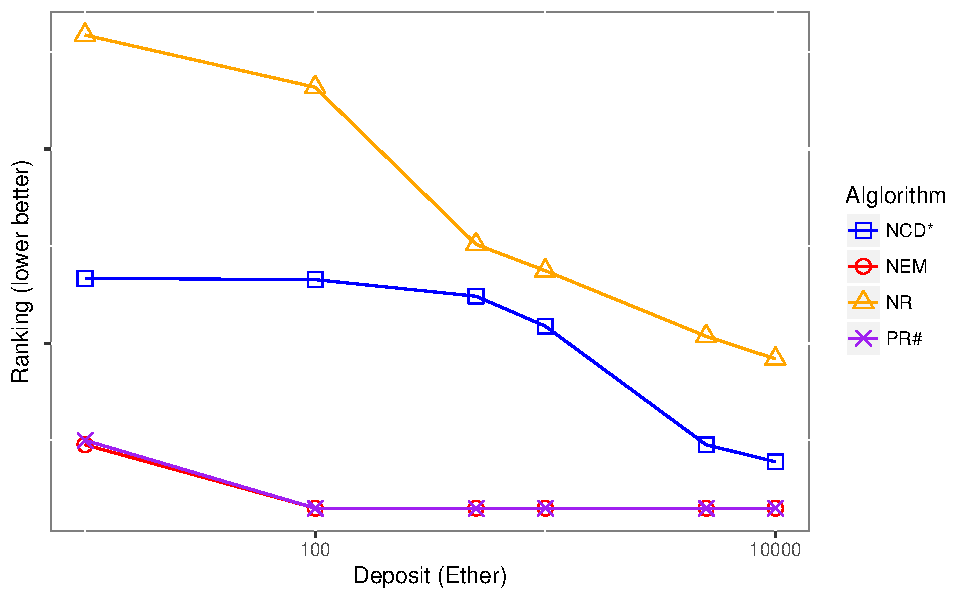
\includegraphics[width=0.7\textwidth]{figs/AttackDeposit.pdf}
		\caption{攻击次数固定为5000次, 攻击投入本金对排名的影响 \\ \footnotesize{(横纵坐标均为对数形式)}}
		\label{subfig:deposit}
	\end{subfigure}
	
	\begin{subfigure}{\linewidth}
	    \centering
		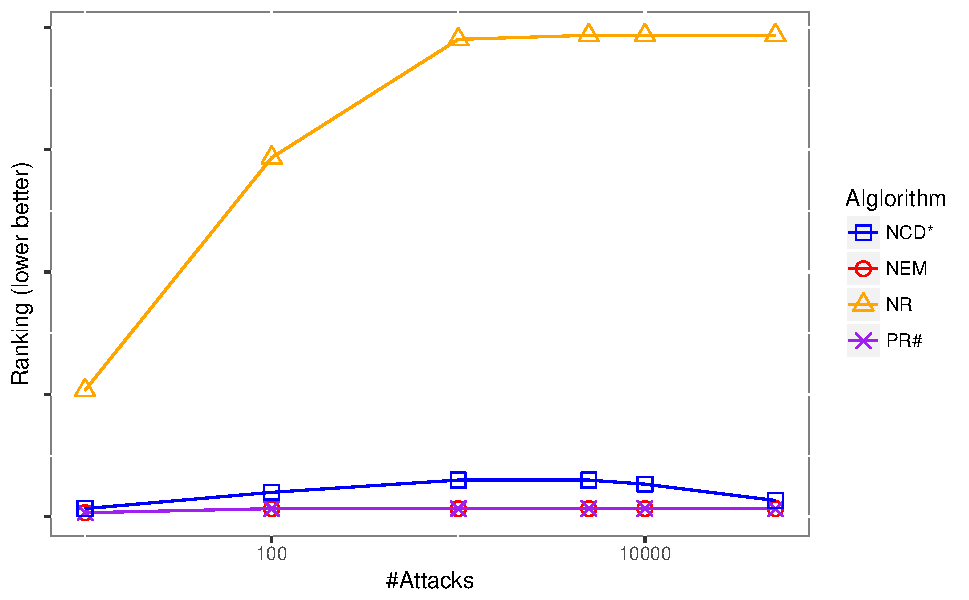
\includegraphics[width=0.7\textwidth]{figs/AttackTimes.pdf} 
		\caption{攻击投入本金固定为$\Xi5000$, 攻击次数对排名的影响  \\ \footnotesize{(横坐标为对数形式)}}\label{subfig:times}
	\end{subfigure}

	\caption{抗操纵测试结果} \label{fig:antiManipulation}
	\caption*{\footnotesize{攻击方式如\reffig{fig:loop}所示,横轴为攻击成本,纵轴为攻击者主节点的排名(排名越靠后纵坐标越高,算法抵抗操纵能力越好) \\
	NR:交易图如\refsec{subsec:txg}所述,排名算法按照\refsec{subsec:leaderrank}所述;\\PR$^*$:交易图如\refsec{subsec:txg}所述,PageRank排名算法;\\ NCD$^*$:交易图如\refsec{subsec:txg}所述,NCDawareRank排名算法;\\ NCD$^{\#}$:交易图如\cite{nem}所述,NCDawareRank排名算法;\\ PR$^{\#}$:交易图如\cite{nem}所述,PageRank排名算法 \\ PageRank的damping factor为0.15;NCDawareRank使用pscan\cite{chang2017mathsf}社群划分算法,$\eta=0.75$, $\mu=0.1$}}
\end{figure}

\subsection{Related Works} \label{subsec:related}

Centrality, the core ranking index, is a most studied concept in network science since decades ago\cite{newman2010networks}. There are a body of literatures introducing various centralities, including degree centrality\cite{freeman1979set}, eigenvector centrality\cite{bonacich1972factoring}, Katz centrality\cite{katz1953new}, closeness centrality\cite{sabidussi1966centrality}, betweenness centrality\cite{freeman1977set}\cite{freeman1978centrality}\cite{freeman1991centrality}\cite{noh2004random}\cite{newman2005measure}, PageRank\cite{Brin2010}, HITS\cite{kleinberg1999authoritative}, SALSA\cite{Science2001}, etc. Besides, there are some fundamental works trying to clearly classify and review these measurements by a unified framework\cite{Borgatti2005}\cite{Borgatti2006}\cite{Lu2016}. When designing \textbf{Nebulas Rank}, before proper centrality is adopted, first we need to consider the property of graph. Blockchain transaction graph's scenario is most similar to the money exchange flow network mentioned in \cite{Borgatti2005}. But the related algorithms mentioned by their work, such as flow betweenness centrality\cite{freeman1991centrality} and random-walk betweenness centrality (aka. current betweenness centrality)\cite{newman2005measure}, are compute intensive and do not satisfy the property of "computable" with the large scale of Blockchain transaction graph.

Since Bitcoin\cite{Nakamoto2008} system released in 2009, researchers have done some statistical and empirical analysis on Bitcoin's transaction graph\cite{Ron}\cite{Haslhofer}\cite{NielKondor2014}\cite{Baumann2014}, and some use the transaction graph structure to discuss anonymity in Bitcoin\cite{Meiklejohn2013}\cite{Ober2013}\cite{pham2016anomaly}\cite{Fleder2015}\cite{Ferrin2015}. After other cryptocurrencies emerged and become popular, transaction graph analysis is conducted with more blockchains\cite{Chang2017}\cite{Anderson2016}. \textbf{Nebulas Rank} adopts their transaction graph concept, i.e. Entity Graph in \cite{Tschorsch2015}, with minor revisions. That is, each account, or set of accounts belonging to the same people, is mapped as a node. And each directed edge represents the intensity of transferring between two accounts. Actually before blockchain system like Bitcoin was invented, scientists have tried to study some financial networks among banks and global trading entities\cite{propper2008towards}\cite{Boss2004}\cite{Serrano2007}\cite{Bech2008}\cite{Fagiolo2009}\cite{Morten2006}\cite{Boss2004a}\cite{Krempel2002}\cite{Serrano2003}. Comparing with blockchain transaction graph, these early studied finical networks are defined not only by transferring activities, but also by extra information such as loan. Moreover, the scale of these networks is much smaller. To conclude, there is rarely research work proposing custom ranking method for large scale transaction graph, especially blockchain transaction graph.

The most relevant work with \textbf{Nebulas Rank} is NEM\cite{nem}'s Proof-of-Importance scheme. It adopts NCDawareRank\cite{Nikolakopoulos2013}, which exploits the clustering effect of network topology, as the ranking algorithm, with clustering algorithm based on SCAN algorithm\cite{xu2007scan}\cite{shiokawa2015scan}\cite{chang2017mathsf}. Although community structure does exist in transaction graph and should be helpful to handle with spam nodes, it does not guarantee that all nodes in Blockchain world controlled by one entity in the real world are mapped into one cluster, which leads to large room for manipulation. Besides, \textcite{Fleder2015} uses PageRank\cite{Brin2010}\cite{page1999pagerank} as an assisting metric to discover interesting addresses and analyze their activities. However, their work does not provide an automated framework to identify important nodes. Instead, it still relies on subjective analyzing, which does not match \textbf{Nebulas Rank}'s context. The algorithm we choose is LeaderRank\cite{Chen2013}\cite{Li2014}. It is a simple yet effective variant of PageRank\cite{Brin2010}\cite{page1999pagerank}. In PageRank, every node is assigned with identical teleportation parameter, while LeaderRank adds a ground node, assigning different teleportation parameter for each node. The weighing scheme of \textbf{Nebulas Rank} is partly from \textcite{Li2014}'s design, which allows nodes with more in-degree to be more likely visited by teleportation. Adopting LeaderRank algorithm could yield results more suitable for the scenario of Blockchain.

